\chapter{Full Datapath}


\section{Datapath}
You are ready to assemble the full non-pipelined datapath shown in Fig~\ref{fig:datapath}.  To do this, you will need to combine all 5 stages into datapath.v.  Stages include:
\begin{enumerate}
\item iFetch
\item iDecode
\item iExecute
\item iMemory
\item iWriteBack
\end{enumerate} 

Verify by running your set of instructions in fibI.data and testing the output.  Each instruction should execute as expected according to your Expected Results Table.  Datapath.v should be your top-level Verilog file (no additional test drivers are necessary).

You should also verify correct operation by creating a new set of datafiles to implement the division code shown below.  You should first write assembly code, then translate it into binary.  One restriction is that the only non-zero value in your fibR.data should be for X22, which can be used as the base address for the array A.  Otherwise, all other data must be loaded from memory via the fibD.data and LDUR commands.  Please pay attention to the comments in division.c.

\Verilog{C code for doing simple division.}{code:division}{../code/division.c}

\begin{figure}
\caption{Full Non-Pipelined Datapath}\label{fig:datapath}
\begin{center}
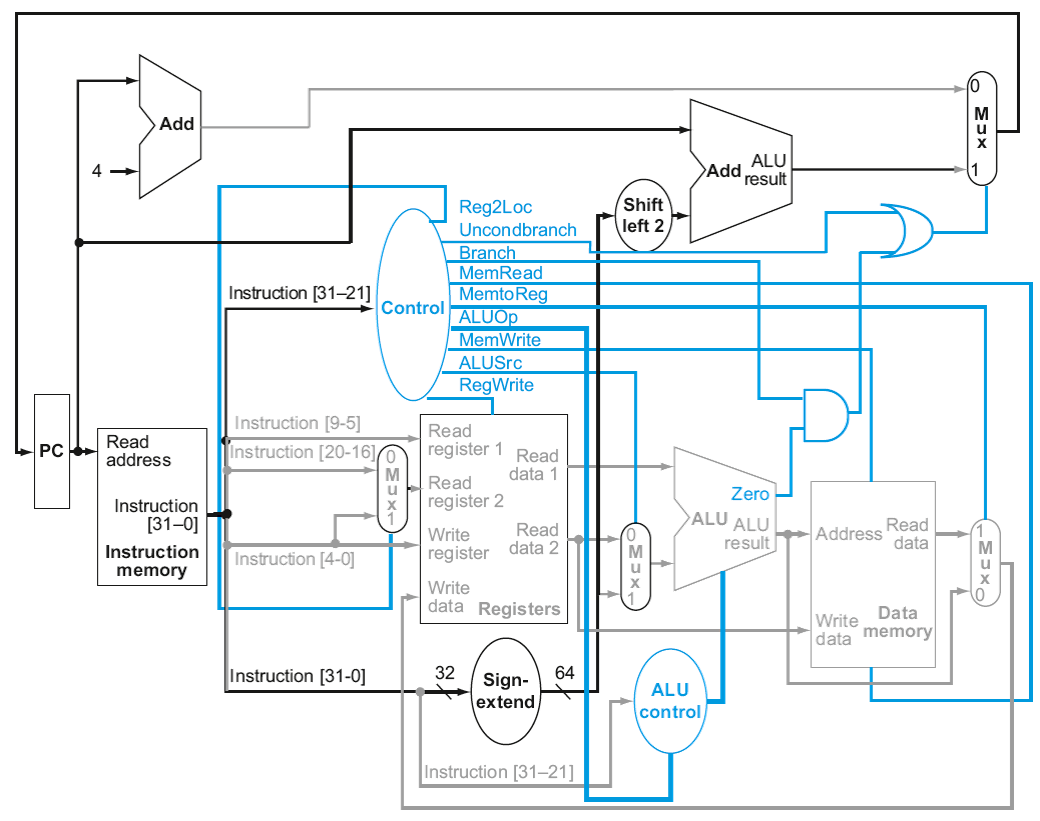
\includegraphics[width=\textwidth]{../images/non_pipelined_datapath.png}
\end{center}
\end{figure}

\section{Your Assignment}

You are to:
\begin{enumerate}
\item Integrate all five stages into the file pipeline.v.
\item Run simulations to verify that your results match your Expected Results table.   
\item Implement the assembly and binary code for the Division C Code shown above.
\item Verify that the divison works correctly.
\item Write up a lab report according to a new format file, LabWriteup.tex.
\end{enumerate} 